\documentclass[10pt]{article}
\usepackage{fullpage}
\usepackage{enumitem}
\usepackage{amsmath}
\usepackage{amssymb}
\usepackage{graphicx}
\usepackage[T1]{fontenc}
\usepackage{lipsum}
\usepackage{listings}
\usepackage{float}
\usepackage{scrextend}
\usepackage{hyperref}
\usepackage{algorithm}
\usepackage{algpseudocode}
\usepackage{tikz}
\usetikzlibrary{arrows,
                backgrounds,
                fit,
                positioning,
                quotes,
                shapes}


\newenvironment{subs}
  {\adjustwidth{3em}{0pt}}
  {\endadjustwidth}

\title{\vspace{-1cm} \Huge Project 3 - Encore Airlines\\ \LARGE CmpE 250, Data Structures and Algorithms, Fall 2022 }
\author{
  Instructor: Özlem Durmaz \.{I}ncel\\
  TAs: Suzan Ece Ada, Bar{\i}\c{s} Yamansavaşç{\i}lar\\
  SAs:  Batuhan \c{C}elik, Bahad{\i}r Gezer, Zeynep Buse Ayd{\i}n, Ömer Faruk Ünal \\
  Contact Address: \href{mailto:bahadirgezerbg@gmail.com}{bahadirgezerbg@gmail.com} 
}
\date{Due: 30/11/2022, 23:55 Sharp}


\begin{document}
  \maketitle
  \vspace{0.05cm}
  
\section{Introduction}

\indent \indent Aviation makes the dream and desire of being able to fly a reality. A strong and affordable global air transport network transcends continents, greatly expands local access to foreign supplies and markets, provides invaluable opportunities for cultural and social exchange, and enhances emergency and humanitarian response capabilities during crises and public health emergencies. All these opportunities and many more depend on the flawless execution of our flight operations. 
\\\\
\indent Air traffic management is a cooperative, international effort and does not stop at borders, on land or in the air. International cooperation of air traffic control providers has helped make commercial aircraft one of the most rapid and dependable mode of travel. Flight operations staff work around the clock to ensure the smooth running of these services. In this project, you will explore these flight operations services' event-driven flight scheduling and processing routines.


\section{Details}

\indent \indent In this project you will simulate an air traffic management system. This system has area control centers, air traffic controllers, airports and flights. Area control centers are where flights enter and exit the simulation. Each area control center has a set of airports its' responsible for and each airport has one air traffic controller. These air traffic controllers are what the area control center will communicate with when processing flight events. Your job is to make sure that each flight is handled correctly. 

\begin{quote}
    
\subsection{\large\textbf{ACC}}
    \begin{itemize}
    
    \item Area control center, or ACC, is the entry and exit point for flights.
    
    \item Area control centers are identified by a unique code consisting of 4 capital letters. 
    
    \item Each area control center is responsible for a set of airports. Every airport has one and only one air traffic controller. This air traffic controller communicates with the area control center. The area control center will delegate the departure and landing phases of the flight to the air traffic controller. Control will be given back to the area control center when these phases are done.
    
    \item There might be more than one area control center. These area control centers are completely independent. They have their own flights, their own airports, and their own air traffic controllers for those airports. In other words, a flight or an airport or an air traffic controller can only be a part of one area control center. 
    
    \item Every airport in an area control center is connected to every other airport in that area control center. 
    
    \item Flights can only fly between airports in the same area control center. Passages between area control centers do not happen. 
    
    \item Flights need to have some operations done by the area control center to progress forward. At any given time there might be more than one flight that needs their operation done. These flights will form a queue while the area control center is busy. This queue is called the ready queue, because it holds flights that are ready to be processed by the area control center. 
    \\ \\
    Area control centers are almost always really busy, but each flight should also have a good response time to ensure the smooth running of flight operations. To this end, the area control center will process the first flight in the ready queue, however, this flight will only be processed for some predetermined time-slice. If the operations do not finish in the given time-slice, the flight is sent all the way to the back of the queue for further processing; else, if the operations finish the flight continues on with its' next step. 
    \\ \\
    There might be cases where two flights want to enter the ready queue at the same time. In such a case, if one of the flights is new to the queue and the other one just finished processing and got sent to the back of the queue, the new one has priority. If the both flights are new, then the flight with the lower flight code, by string comparison, has higher priority. 
    \\ \\ 
    Area control centers in this air traffic management system use a time-slice of 30 units of time. The chart below visualizes this time-slice processing regime. Flight entries are flight codes followed by the amount of time needed to finish that flight. 
    \end{itemize}
    
\begin{center}
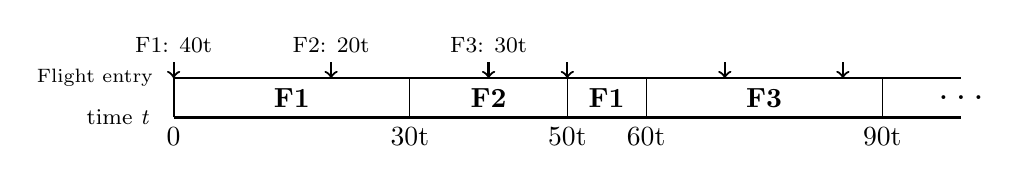
\begin{tikzpicture}[scale=1]
    \draw[thick, color=black] (0,0) node[anchor=north] {{0}} -- (10,0);
    \draw[thick, color=black] (0,0.5) -- (10,0.5);
    \draw[thick, color=black] (0,0) -- (0,0.5);
    %\draw[thick, color=black] (10,0) -- (10,0.5);
    
    \draw[thick, ->] (0, 0.7) node[anchor=south] {\footnotesize{F1: 40t}} -- (0,0.5);
    
    \draw[thick, ->] (2, 0.7) node[anchor=south] {\footnotesize{F2: 20t}} -- (2,0.5);
    
    \draw[thick, ->] (4, 0.7) node[anchor=south] {\footnotesize{F3: 30t}} -- (4,0.5);
    
    \draw[thick, ->] (5, 0.7) -- (5,0.5);
    \draw[thick, ->] (7, 0.7) -- (7,0.5);
    \draw[thick, ->] (8.5, 0.7) -- (8.5,0.5);
    
    \node[align=center] at (1.5,0.25) {\textbf{F1}};
    \node[align=center] at (4,0.25) {\textbf{F2}};
    \node[align=center] at (5.5,0.25) {\textbf{F1}};
    \node[align=center] at (7.5,0.25) {\textbf{F3}};
    \node[align=center] at (10,0.25) {\Large{\textbf{$\mathbf{\dots}$}}};
    
    \draw (3, 0) node[anchor=north] {30t} -- (3, 0.5);
    \draw (5, 0) node[anchor=north] {50t} -- (5, 0.5);
    \draw (6, 0) node[anchor=north] {60t} -- (6, 0.5);
    \draw (9, 0) node[anchor=north] {90t} -- (9, 0.5);
    
    \node[align=right] at (-0.7,0) {\footnotesize{time \textit{t}}};
    \node[align=right] at (-1, 0.5) {\scriptsize{Flight entry}};
     
\end{tikzpicture}
\end{center}


\subsection{\large\textbf{ATC}}

    \begin{itemize} 
    
    \item Air traffic control, or ATC, is an auxiliary flight manager. 
    
    \item Each air traffic control is responsible for a single airport. 
        
    \item Flights taking off from or landing at an airport need their operations done by the air traffic controller for that airport. So, when time comes, the area control center will delegate flights to the required air traffic controller. When the take off or land operations end, the air traffic controller will control of the pass the flight back to the area control center. 
    
    \item At any given time air traffic control might have more than one flight that needs their operation done, just like the area control center. These flights will again form a queue called the ready queue. Air traffic controllers are also very busy, however, unlike the area control center, air traffic control must commit to one flight when it starts processing it. So the first flight in the queue will be processed first, and it will be processed until the completion of its' operations. 
    
    \item Air traffic controllers are identified by a unique code consisting of 7 characters, the first 4 characters of which is the area control center code it belongs to, the following 3 characters are numbers from $0$ to $999$, filled with zeros from the front. 
    \\ \\ 
    These numbers are obtained by placing the airport code of this air traffic control into an available slot in a table of size $1000$. Every area control center will have its' own table, filled with airports it is responsible for. For every $i$th character of the airport code string, $i$ starting from zero of course, the ASCII value for that character will be multiplied by $31^{i}$. These $i$ multiplications will be summed together to generate the initial slot value. Search for an available slot will start from the position denoted by the last three digits of the initial slot value. If a slot is not available, the next slot will be considered. If the end of the table is reached jump back to the beginning slot of the table and continue. There will not be more than $1000$ airports in one area control center, and consequently in one table, so every airport will eventually find a slot. Air traffic control codes are generated in the order their respective airport code appears in the input. 
    
    \end{itemize}
    
\subsection{\large\textbf{Flight}}
    
    
    \begin{itemize}

    \item Flights are the entities that needs processing. 
    
    \item Each flight has a departure and landing airport, both airports belong to the same area control center. Which area control center these airports belong to will be given in the input.
    
    \item A flight has 21 operation steps to complete before termination. These steps and their order are explained in detail in the next section. Durations of these steps will be given in the input. 
    
    \item Flights enter and exit the simulation through the area control center. In the area control center flights process their operation steps until termination. These processing steps repeat a certain form. This form can be visualized as a collection of states the flight can be in. A state diagram is given below to help you visualize the situation.
    
    \item During processing the flight event will cycle through the states. Twice during these cycles, the flight will exit states that belong to the area control center and enter states that belong to an air traffic control, where it will process either the departure or the landing operation steps of the flight. After the air traffic control has cycled through its' states, the flight will be back in the area control center states, and it will continue processing from there. 

    \end{itemize}

%\vspace{1cm}
\begin{center}
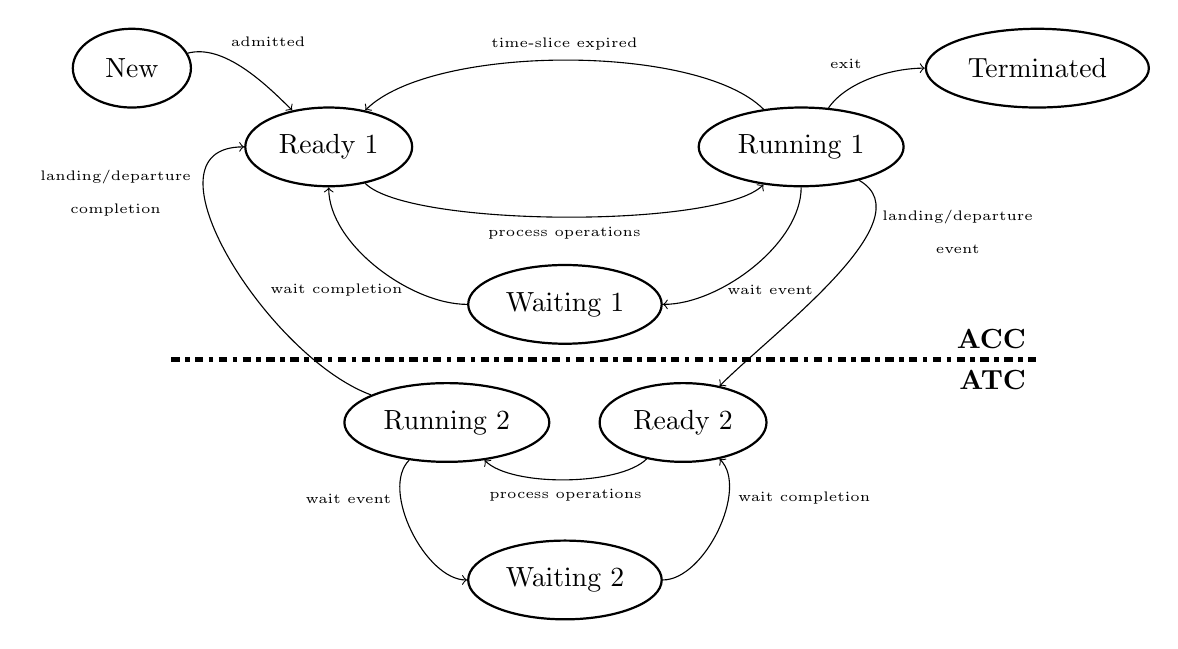
\begin{tikzpicture}[scale=1]

%\draw[thick] (-7,-0.65) -- (8,-0.65) node[anchor=north] {ACC} node[anchor=south] {ATC};

\draw[ultra thick, color=black, dash dot] (-5,-0.7) -- (6,-0.7) 
node[anchor=south east] {\textbf{ACC}} node[anchor=north east] {\textbf{ATC}};

\begin{scope}[opacity=0.1]
    %\draw[rounded corners] (-7, -0.6) rectangle (8, 4) [fill=blue] {};
    %\draw[rounded corners] (-7, -5.5) rectangle (8, -0.7) [fill=red] {};
\end{scope}  

\begin{scope}[ res/.style = {ellipse, draw, minimum height=1cm, minimum width=1.5cm}, thick]
    \node[res] (1) at (6, 3) {Terminated};
    \node[res] (2) at (-5.5, 3) {New};
    \node[res] (3) at (3,2) {Running 1};
    \node[res] (4) at (0,0) {Waiting 1};
    \node[res] (5) at (-3, 2) {Ready 1};
    
    %\node[res] (6) at (2.5, -1.5) {New};
    %\node[res] (7) at (-2.5, -1.5) {Terminated};
    \node[res] (8) at (1.5, -1.5) {Ready 2};
    \node[res] (9) at (0, -3.5) {Waiting 2};
    \node[res] (10) at (-1.5, -1.5) {Running 2};
\end{scope}

%    \draw [->] (0,0) -- (5,0) node [midway, below] {Text};
%    \draw [->] (0,1) -- (5,1) node [near end, below] {Text};
%    \draw [->] (0,2) -- (5,2) node [pos=0.62, below] {Text};
%    \draw [->] (0,3) -- (5,3) node [pos=0.2, below] {Text};
%   node[label= below:text] {}


\begin{scope}
    \draw[->] (2) to [out=15, in=135, looseness=.8] node[pos=0.3, above right] {\tiny{admitted}} (5); 
    \draw[->] (3) to [out=55, in=180, looseness=.8] node[pos=0.5, above left] {\tiny{exit}} (1); 
    \draw[->] (3) to [out=135, in=45, looseness=.6] node[pos=0.5, above] {\tiny{time-slice expired}} (5); 
    \draw[->] (5) to [out=-45, in=225, looseness=.4] node[pos=0.5, below] {\tiny{process operations}} (3); 
    \draw[->] (3) to [out=270, in=0, looseness=.8] node[pos=0.7, right] {\tiny{wait event}} (4); 
    \draw[->] (4) to [out=180, in=270, looseness=.8] node[pos=0.3, left] {\tiny{wait completion}} (5); 
    
    \draw[->] (3) to [out=-30, in=45, looseness=0.8] node[pos=0.3, right, text width=2cm, align=center] {\tiny{landing/departure event}} (8); 
    \draw[->] (10) to [out=160, in=180, looseness=1] node[pos=0.7, left, text width=2cm, align=center] {\tiny{landing/departure completion}} (5); 
    
    %\draw[->] (10) to [out=180, in=200, looseness=.9] (7); 
    %\draw[->] (6) to [out=-45, in=0, looseness=.8] (8); 
    %\draw[->] (10) to [out=45, in=135, looseness=.6] node[pos=0.5, above] {\tiny{interrupt}} (8); 
    \draw[->] (8) to [out=225, in=-45, looseness=.6] node[pos=0.5, below] {\tiny{process operations}} (10); 
    \draw[->] (9) to [out=0, in=-45, looseness=.8]  node[pos=0.7, right] {\tiny{wait completion}} (8); 
    \draw[->] (10) to [out=225, in=180, looseness=.8] node[pos=0.3, left] {\tiny{wait event}} (9); 
\end{scope}

\end{tikzpicture}
\end{center}
%\vspace{1cm}

\subsection{\large\textbf{Operation Times}}

Every flight will follow a certain chain of states. Each state needs some amount of time to complete its' operation. These state chains are given below, in order. Operation times will be given for each running and waiting state in the input. The completion of running states depend on the availability of either the area control center or the air traffic control responsible for the execution. So, time spent in the ready states depends on the scheduling situation. Waiting states just require the flight to wait for a certain amount of time before continuing with the next operation. 

\begin{itemize}
    \item[] \textbf{ACC - Running: } ACC initial processing.
    \item[] \textbf{ACC - Waiting: } Relaying flight information to ACC.
    \item[] \textbf{ACC - Running: } Control transfer from ACC to departure ATC. 
    \item[] \textbf{ATC Departure - Running: } Departure ATC initial processing. 
    \item[] \textbf{ATC Departure - Waiting: } Boarding wait.
    \item[] \textbf{ATC Departure - Running: } Taxi information processing.
    \item[] \textbf{ATC Departure - Waiting: } Taxi wait.
    \item[] \textbf{ATC Departure - Running: } Takeoff clearance processing.
    \item[] \textbf{ATC Departure - Waiting: } Takeoff wait.
    \item[] \textbf{ATC Departure - Running: } Control transfer from departure ATC to ACC.
    \item[] \textbf{ACC - Running: } Flight path processing.
    \item[] \textbf{ACC - Waiting: } Flight wait.
    \item[] \textbf{ACC - Running: } Control transfer from ACC to arrival ATC. 
    \item[] \textbf{ATC Arrival - Running: } ATC initial processing and landing clearance processing. 
    \item[] \textbf{ATC Arrival - Waiting: } Landing wait.
    \item[] \textbf{ATC Arrival - Running: } Taxi information processing.
    \item[] \textbf{ATC Arrival - Waiting: } Taxi wait.
    \item[] \textbf{ATC Arrival - Running: } Gate and ground crew information processing.
    \item[] \textbf{ATC Arrival - Waiting: } Disembarkation wait. 
    \item[] \textbf{ATC Arrival - Running: } Control transfer from arrival ATC to ACC.
    \item[] \textbf{ACC - Running: } ACC wrap-up. 
\end{itemize}

\end{quote}


\section{Input \& Output}

\begin{quote}

\subsection{Input}
\begin{quote}
Input file path will be given as the first program argument. \\

\iffalse
Input file format:
    1. First line: <number of ACCs> <number of flights>
    2. Next <number of ACCs> lines: <ACC code> <airport code> <airport code> ... <airport code>
    3. Next <number of flights> lines: <admission time> <flight code> <ACC code> <departure airport code> <arrival airport code> <list of operation times>
\fi

\vspace{-0.2cm}
\\ \medium{\textbf{Format}} \\
Input begins with a single line containing two space-separated integers $A$ and $F$. Then, $A$ lines follow, the $i$th of which contains space-separated codes starting with $A_{i}$ the ACC code, followed by airport codes connected to that ACC, $j$th of which is $H_{ij}$. Then, $F$ lines follow, the $k$th of which contains 26 space-separated values, $T_{k}$ admission time, $F_{k}$ the flight code, $A_{k}$ ACC code, $O_{k}$ departure airport code, $D_{k}$ arrival airport code, respectively. Followed by 21 space-separated integers, denoting the operation times for the flight $F_{k}$, $m$th of these operation times is $P_{km}$. \\

\goodbreak
\vspace{-0.2cm}
\\ \medium{\textbf{Constraints}} \\
$1 \leq A, i \leq 10^{4} \\ 
$1 \leq F, k \leq 6 \cdot 10^{6} \\
$0 \leq T_{k} \leq 10^{9}$ \\
$2 \leq j \leq 1000$ \\ % max number of airports in an ACC
$1 \leq m \leq 21$ \\ % number of process/ wait times
$1 \leq P_{km} \leq 500$ \\ % processing time
$A_{i}, A_{k} \in [$\texttt{"AAAA"-}\texttt{"ZZZZ"}$]$ \\
$O_{k}, D_{k}, H_{ij} \in [$\texttt{"AAA"-}\texttt{"ZZZ"}$]$ \\
$F_{k} \in [$\texttt{"AA1111"-}\texttt{"ZZ9999"}$]$ 
\end{quote}

\subsection{Output}
\begin{quote}
Output file path will be given as the second program argument. \\

\vspace{-0.2cm}
\\ \medium{\textbf{Format}} \\
The output will consist of $A$ lines, one for each ACC. Ordering between ACC lines does not matter. Each ACC line has an ACC code followed by a space-separated integer denoting the time of termination of the last flight. The next $j$ space-separated strings are airport codes and their slot concatenated together. These values are for each ACC. 

\end{quote}

\end{quote}

\section{Submission}

\indent \indent Your project will be graded automatically. So it's important that you carefully follow the submission instructions. First, all of your source files, and nothing more, should be collected under \verb|Project3/src|. Then, you should zip the \verb|Project3| folder and rename it to \texttt{p3\_<student$_{id}$>.zip} (e.g., \verb|p3_2020400999.zip|). This zip file will be submitted through moodle. These steps should be followed in order. \\

Your program must be runnable through the terminal. We will compile your code with the \texttt{javac} command. The target version is 17. Hence, it is imperative that your project structure is correct, otherwise you will not be able to get any points from the automatic grading system.  The compiled program will be run using \texttt{java} command. Your program should be able to run with full-path arguments.

\section{Grading}

\indent \indent Grading of this project is based on the automatic compilation and run and the success of your code in test cases. If your code compiles and runs with no error, then you will get 10\% of the project grade. 90\% of your grade will be the sum of points collected from each input/output test case. Each test case will have equal weight. Outputs will have partial grading, each correct ACC line will contribute towards your final grade. Wrong values do not reduce your grade. Maximum project grade is 100\%. 

\section{Warnings}

\begin{itemize}

\item This is an individual project. 

\item All source codes are checked automatically for similarity with other submissions and exercises from previous years. Make sure you write and submit your own code. Any sign of cheating will be penalized by at least -50 points at first attempt and F grade in case of recurrence.

\item Make sure you document your code with necessary inline comments and use meaningful variable names. Do not over-comment, or make your variable names unnecessarily long. This is very important for partial grading.

\item Do not start coding right away. Think about the structure of your program and the possible complications resulting from it before coding.

\item Make sure that the white-spaces in your output is correct. You can disregard the ones at the end of the line.

\item Questions about the project should be sent through the contact address in the first page.

\item There will be a time limit of 60 seconds for your program execution. This is not a strict time limit, execution times may vary for each run, thus objections regarding to time limits will considered if necessary. 

\end{itemize}



\end{document}